% Options for packages loaded elsewhere
\PassOptionsToPackage{unicode}{hyperref}
\PassOptionsToPackage{hyphens}{url}
%
\documentclass[
]{article}
\usepackage{amsmath,amssymb}
\usepackage{lmodern}
\usepackage{iftex}
\ifPDFTeX
  \usepackage[T1]{fontenc}
  \usepackage[utf8]{inputenc}
  \usepackage{textcomp} % provide euro and other symbols
\else % if luatex or xetex
  \usepackage{unicode-math}
  \defaultfontfeatures{Scale=MatchLowercase}
  \defaultfontfeatures[\rmfamily]{Ligatures=TeX,Scale=1}
\fi
% Use upquote if available, for straight quotes in verbatim environments
\IfFileExists{upquote.sty}{\usepackage{upquote}}{}
\IfFileExists{microtype.sty}{% use microtype if available
  \usepackage[]{microtype}
  \UseMicrotypeSet[protrusion]{basicmath} % disable protrusion for tt fonts
}{}
\makeatletter
\@ifundefined{KOMAClassName}{% if non-KOMA class
  \IfFileExists{parskip.sty}{%
    \usepackage{parskip}
  }{% else
    \setlength{\parindent}{0pt}
    \setlength{\parskip}{6pt plus 2pt minus 1pt}}
}{% if KOMA class
  \KOMAoptions{parskip=half}}
\makeatother
\usepackage{xcolor}
\IfFileExists{xurl.sty}{\usepackage{xurl}}{} % add URL line breaks if available
\IfFileExists{bookmark.sty}{\usepackage{bookmark}}{\usepackage{hyperref}}
\hypersetup{
  hidelinks,
  pdfcreator={LaTeX via pandoc}}
\urlstyle{same} % disable monospaced font for URLs
\usepackage[margin=1in]{geometry}
\usepackage{graphicx}
\makeatletter
\def\maxwidth{\ifdim\Gin@nat@width>\linewidth\linewidth\else\Gin@nat@width\fi}
\def\maxheight{\ifdim\Gin@nat@height>\textheight\textheight\else\Gin@nat@height\fi}
\makeatother
% Scale images if necessary, so that they will not overflow the page
% margins by default, and it is still possible to overwrite the defaults
% using explicit options in \includegraphics[width, height, ...]{}
\setkeys{Gin}{width=\maxwidth,height=\maxheight,keepaspectratio}
% Set default figure placement to htbp
\makeatletter
\def\fps@figure{htbp}
\makeatother
\setlength{\emergencystretch}{3em} % prevent overfull lines
\providecommand{\tightlist}{%
  \setlength{\itemsep}{0pt}\setlength{\parskip}{0pt}}
\setcounter{secnumdepth}{-\maxdimen} % remove section numbering
\ifLuaTeX
  \usepackage{selnolig}  % disable illegal ligatures
\fi

\author{}
\date{\vspace{-2.5em}}

\begin{document}

\hypertarget{sistrat-datasets}{%
\section{SISTRAT Datasets}\label{sistrat-datasets}}

Welcome to the repositories of the construction of the treatment
information system (SISTRAT) datasets. On this repository you can find
the different processes and actions taken to standardize and prepare the
data for the analysis of the investigators of the project.

This page is composed by the following main topics:

\begin{enumerate}
\def\labelenumi{\arabic{enumi}.}
\item
  \href{Encript.html}{Encryption of RUTs and Generation of HASHs}
\item
  \href{Data_prep_C1}{Data Preparation and Standardization of C1}

  1.1. \href{SER_Stata.html}{Preliminary Results for SER 2020}

  1.2. \href{Duplicates}{Deduplication of C1}

  1.3. \href{Duplicates2}{Deduplication of C1, Part 2}

  1.4. \href{Duplicates3}{Deduplication of C1, Part 3}

  1.5. \href{Duplicates4}{Deduplication of C1, Part 4}

  1.6. \href{Presentación2}{Presentation of Preliminary Processes and
  Descriptive Data to Institutions}

  1.7. \href{Desc}{Descriptive Glimpse of the Database}

  1.8. \href{codebook}{Codebook of C1}
\item
  Associations \& Analytic Exercises

  3a.1. Ambulatory or residential? a multi-state analysis of treatments
  for substace use disorders- Main analyses

\begin{verbatim}
 3a.1.1.a [Step 1: Imputation, Matching & set the database](Matching_Process1_APR_22)

 3a.1.1.b [Stata, Step 1: Set the database, AJ estimates, Compute Transition Probabilities](Matching_Process1_stata_APR_22)

 3a.1.2.b [Stata, Step 2: Compute Transition Probabilities at 3 years](Matching_Process2_stata_APR_22)

 3a.1.3.b [Stata, Step 3: Plot probabilities and differences](Matching_Process3_stata_APR_22)

 3a.1.4.b [Stata, Step 4: Compute Transition Probabilities for a patient that completed treatment at 3 years](Matching_Process4_stata_APR_22)

 3a.1.4.5.b [Stata, Step 4.5: Summarise estimates in tables and export](Matching_Process4_5_stata_APR_22)

 3a.1.6.a [Step 5: Sensitivity analyses, Sankey, Transition Trees](Matching_Process5_APR_22) 
\end{verbatim}

  3a.2. Ambulatory or residential? a multi-state analysis of treatments
  for substace use disorders- Supplemental analyses

\begin{verbatim}
 3a.2.1.a [Step 1.25](Matching_Process1_25_APR_22)

 3a.2.2.a [Step 1.5](Matching_Process15_APR_22)

 3a.2.3.a [Step 2)](Matching_Process2_APR_22)

 3a.2.4.a [Step 3)](Matching_Process3_APR_22)

 3a.2.5.a [Step 4)](Matching_Process4_APR_22)

 3a.2.6.b [Stata, Step 5)](Matching_Process5_stata_APR_22)

 3a.2.1.c [Stata, Step 1 w/ only complete cases)](Matching_Process1_stata_APR_22_cc)
\end{verbatim}

  3b.1. Treatment outcome and readmission risk among women in women-only
  versus mixed-gender drug treatment programs in Chile- Main

\begin{verbatim}
 3b.1.1.a [Step 1: Descriptive tables, Partitioned Survival analyses, Competing risks, Select Survival Distributions](Proyecto_carla3)

 3b.1.2.a [Supplemental: Step 2: Compute Transition Probabilities](Proyecto_carla32)

 3b.1.3.a [Supplemental: Step 2: Get Transition Intensities, Compute Transition Probabilities, Comparative Plots, ](Proyecto_carla33)

 3b.4.a [Step 4: After review, Survival distributions revised, Simulate probabilities to get readmitted](Proyecto_carla34)
\end{verbatim}

  3b.2. Treatment outcome and readmission risk among women in women-only
  versus mixed-gender drug treatment programs in Chile- Supplemental

\begin{verbatim}
 3b.2.1.b [Stata, Step 1](Proyecto_carla1_stata_JUN_21)

 3b.2.2.b [Stata, Step 2](Proyecto_carla2_stata_JUN_21)

 3b.2.3.b [Stata, Step 3](Proyecto_carla3_stata_JUN_21)

 3b.2.4.b [Stata, Step 4](Proyecto_carla4_stata_JUN_21)
\end{verbatim}

  3c.1. Living with \href{analisis_joel2}{conslidation}

  3c.2. Living with (Stata)
  \href{analisis_joel_oct_2021_stata1}{conslidation}

  3c.3. Living with (Stata)- \href{analisis_joel_oct_2021_stata2}{Latent
  Class Analysis}

  3c.4. Living with (Stata)-
  \href{analisis_joel_oct_2021_stata3}{Survival Regression}
\item
  \href{Data_prep_TOP}{Data Preparation and Standardization of TOP or
  Profile of Treatment Results}

  4.1. \href{codebook_TOP}{Codebook of TOP}
\item
  \href{Fiscalia_merge}{Chilean prosecutor's office Data merge}
\item
  \href{https://youtu.be/xuROIbzEw5I}{Webinar ``¿Qué sabemos de los
  programas de tratamiento de drogas en Chile? (What do we know about
  Chilean substance use treatments?)}
\end{enumerate}

The main processes are summarized in the following figures.

\hypertarget{figure-1.-diagram-of-data-preparation}{%
\subparagraph{Figure 1. Diagram of data
preparation}\label{figure-1.-diagram-of-data-preparation}}

To open in a new window

\begin{figure}
\centering
\includegraphics{Figures/RUT_Administración.svg}
\caption{Diagram}
\end{figure}

\hypertarget{figure-2.-strobe-diagram}{%
\subparagraph{Figure 2. STROBE Diagram}\label{figure-2.-strobe-diagram}}

To open in a new window

\begin{figure}
\centering
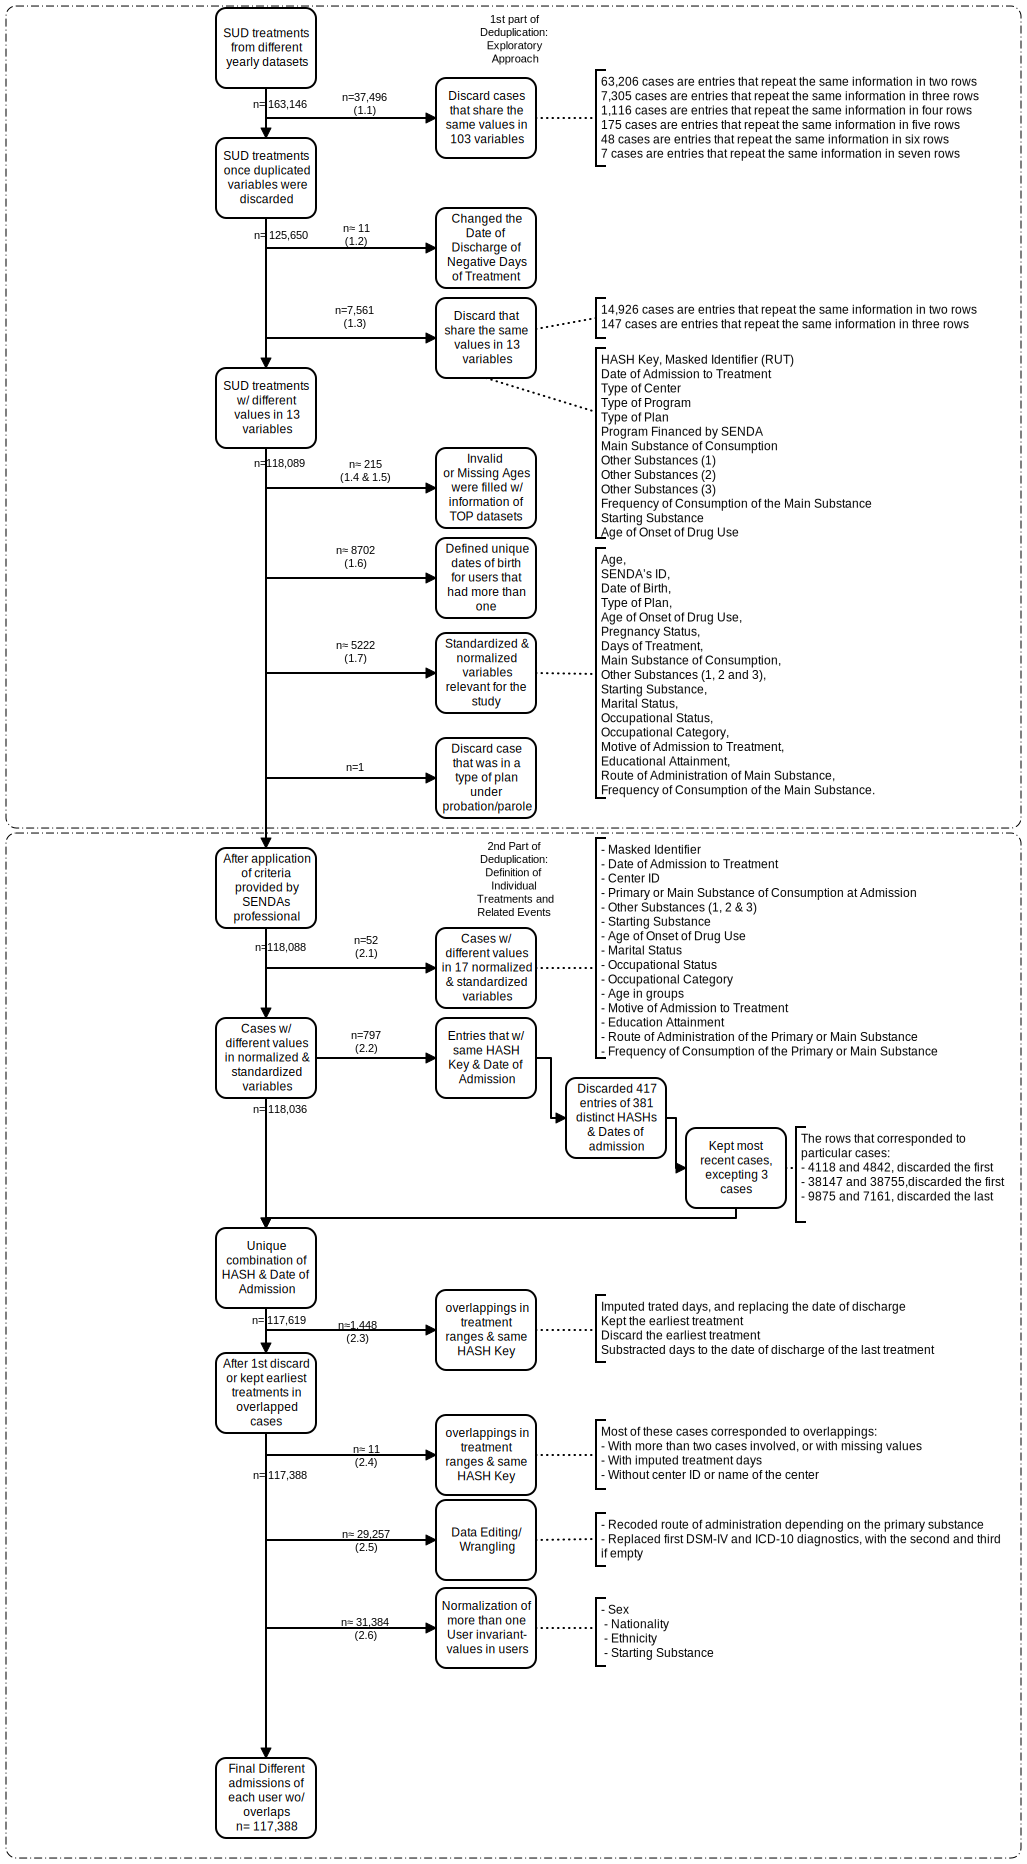
\includegraphics{Figures/Diagram_STROBE.svg}
\caption{STROBE}
\end{figure}

\end{document}
